\documentclass[11pt]{article}
\usepackage[margin=1in]{geometry}
\usepackage{graphicx} % Required for inserting images
\usepackage{amsmath,amssymb,amsthm}
\usepackage{booktabs}
\usepackage{array}
\usepackage{pgfplots}
\pgfplotsset{compat=1.17}
\usepackage[hidelinks]{hyperref}

\newtheorem{theorem}{Theorem}[section]
\newtheorem{proposition}[theorem]{Proposition}
\newtheorem{lemma}[theorem]{Lemma}
\newtheorem{conjecture}[theorem]{Conjecture}
\theoremstyle{definition}
\newtheorem{definition}[theorem]{Definition}
\newtheorem{example}[theorem]{Example}
\theoremstyle{remark}
\newtheorem{remark}[theorem]{Remark}

\newcommand{\F}{F}
\newcommand{\nc}[1]{\langle\!\langle #1 \rangle\!\rangle}
\newcommand{\pres}[2]{\langle #1 \mid #2 \rangle}
\newcommand{\Aut}{\operatorname{Aut}}
\newcommand{\rot}{\operatorname{rot}}
\newcommand{\Sol}{\mathcal{S}}
\newcommand{\Orc}{\mathcal{O}}
\newcommand{\Fix}{\mathcal{F}}
\newcommand{\W}{\mathcal{W}}
\newcommand{\MS}{\mathrm{MS}}
\newcommand{\SMK}{\mathrm{S20\_MK2}}

\title{Stable AC-personal}
\author{Avigya Paudel}
\date{October 2026}

\begin{document}

\maketitle

\section{Introduction}

This note fixes the definitions behind every search method in AC-SolverX and reports the score of each method on a
common benchmark. Each score is the number of presentations of a fixed set that the method certifies within a stated
budget. Each certificate is a sequence of moves, replayed independently on the input presentation before it is
counted.

\paragraph{Notation.} Let $X=\{x_1,\dots,x_n\}$ and let $\F(X)$ be the free group on $X$. A word over
$X^{\pm1}$ is \emph{freely reduced} if it contains no factor $aa^{-1}$ with $a\in X^{\pm1}$, and \emph{cyclically
reduced} if every cyclic permutation of it is freely reduced. For $w\in \F(X)$, $|w|$ denotes the length of its freely
reduced form. For two generators we write $x,y$. In tables, an upper-case letter denotes an inverse: \texttt{xxxYYYY}
is $x^3y^{-4}$.

\begin{definition}[Balanced presentation]
A \emph{presentation} is a pair $P=\pres{X}{R}$ with $R=(r_1,\dots,r_m)$ a tuple of cyclically reduced words. It
presents the group $G_P=\F(X)/\nc{R}$, where $\nc{R}$ is the normal closure of $R$ in $\F(X)$. $P$ is \emph{balanced}
if $m=n$, and $n$ is its \emph{rank}. The \emph{total length} of $P$ is $\lambda(P)=\sum_{i}|r_i|$. The \emph{trivial
presentation} of rank $n$ is $T_n=\pres{x_1,\dots,x_n}{x_1,\dots,x_n}$.
\end{definition}

\paragraph{Benchmarks.} For $n\ge1$ and $w\in\F(x,y)$ with exponent sum $0$ in $x$, the Miller--Schupp presentation
\[
\MS(n,w)=\pres{x,y}{x^{-1}y^{n}x\,y^{-(n+1)},\;x^{-1}w}
\]
presents the trivial group.
\begin{itemize}
  \item \textbf{MS640} is the set of the $640$ presentations of the $1{,}190$-row Miller--Schupp benchmark that the
  LENGTH greedy of Section~\ref{sec:greedy} solves within $10^6$ pops at cap $24$. Every presentation in MS640 is
  therefore AC-trivial, and a method that fails on a row has failed on a solvable instance.
  \item \textbf{bench60} is a $60$-row subset of MS640 spanning its difficulty bins.
  \item \textbf{ladder200} contains $188$ presentations graded into ten difficulty levels by the node count of the
  LENGTH greedy on record ($144$ Aut-minimal AC19 orbits and $44$ MS640 rows).
  \item \textbf{AC19} is the set of $72{,}779$ representatives of the $\Aut(\F_2)$-orbits of the $156{,}762$
  presentations of the extended AC19 data set.
\end{itemize}

\paragraph{Units.} A \emph{pop} (or \emph{node}) is one removal from the search heap. A budget of $B$ pops is per
presentation, and a failed search is charged all $B$ pops. Path lengths are counted in S-moves
(Definition~\ref{def:smove}) unless stated otherwise. Scores measured in different units (pops, the hybrid's work units)
are not compared with each other.

\subsection{AC conjecture}

\begin{definition}[AC moves]\label{def:ac}
Let $P=\pres{X}{r_1,\dots,r_n}$ be balanced. An \emph{AC move} replaces a single relator $r_i$ and leaves the others
unchanged:
\begin{align*}
&(\mathrm{AC1})\quad r_i\mapsto r_i^{-1};\\
&(\mathrm{AC2})\quad r_i\mapsto r_i\,r_j,\qquad j\neq i;\\
&(\mathrm{AC3})\quad r_i\mapsto u\,r_i\,u^{-1},\qquad u\in\F(X).
\end{align*}
After each move the new relator is freely and cyclically reduced.
\end{definition}

Each move has an inverse composed of moves of the same kinds: $r_i\mapsto r_ir_j^{-1}$ is AC1 on $r_j$, then AC2,
then AC1 on $r_j$. A transposition of two relators is also a composite of AC1 and AC2. Hence the relation
$P\sim_{AC}Q$, meaning that $Q$ is obtained from $P$ by a finite sequence of AC moves, is an equivalence relation.
$P$ is \emph{AC-trivial} if $P\sim_{AC}T_n$.

\begin{lemma}[Invariants]\label{lem:inv}
Let $P\sim_{AC}Q$ be balanced presentations on $X$.
\begin{enumerate}
  \item $\nc{R_P}=\nc{R_Q}$; in particular $G_P\cong G_Q$.
  \item Let $M(P)\in\mathbb{Z}^{n\times n}$ be the exponent-sum matrix, where $M_{ij}$ is the exponent sum of $x_j$ in
  $r_i$. Then $|\det M(P)|=|\det M(Q)|$.
\end{enumerate}
Consequently, an AC-trivial presentation presents the trivial group and satisfies $|\det M|=1$.
\end{lemma}

\begin{proof}
(1) Every move replaces $r_i$ by an element of the normal closure of the current relators, and every move is
invertible. (2) Abelianization maps $r_i$ to row $i$ of $M$. AC1 negates a row, AC2 adds row $j$ to row $i$, and AC3
fixes every row. Each therefore multiplies $M$ on the left by a unimodular matrix. Finally, $M(T_n)=I_n$.
\end{proof}

Neither invariant is sufficient for AC-triviality. Every verifier in the code base checks $|\det M|=1$ independently of
the solver.

\begin{conjecture}[Andrews--Curtis, 1965]
Every balanced presentation of the trivial group is AC-trivial.
\end{conjecture}

The conjecture is open and is generally believed to be false. The standard family of potential counterexamples is
the Akbulut--Kirby family
\[
\mathrm{AK}(n)=\pres{x,y}{x^{n}y^{-(n+1)},\;xyx\,y^{-1}x^{-1}y^{-1}},\qquad n\ge2.
\]
$\mathrm{AK}(2)$ is AC-trivial, and $\mathrm{AK}(3)$ is the standard test case.

\subsubsection{Substitution}

\begin{definition}[Substitution move]\label{def:smove}
For a cyclically reduced word $r$ and $0\le k<|r|$, let $\rot_k(r)$ be $r$ with its last $k$ letters moved to the
front. On a balanced presentation of rank $n$, a \emph{substitution move} (S-move) is a tuple $(i,j,s,k_1,k_2)$ with
$i\neq j$ and $s=\pm1$. It acts by
\[
r_i\;\longmapsto\;\rot_{k_1}(r_i)\cdot\rot_{k_2}\!\big(r_j^{\,s}\big),
\]
followed by free and cyclic reduction. The move is admissible only if the last letter of $\rot_{k_1}(r_i)$ is the
inverse of the first letter of $\rot_{k_2}(r_j^{\,s})$, that is, if the product cancels at the seam.
\end{definition}

\begin{lemma}
Every S-move is a composite of AC moves.
\end{lemma}

\begin{proof}
$\rot_k(r)=c\,r\,c^{-1}$ for a suffix $c$ of $r$, so each rotation is an AC3 move. Replacing $r_j$ by $r_j^{-1}$ is AC1,
and the product is AC2. Undoing the conjugation and the inversion of $r_j$ restores the other relator.
\end{proof}

\begin{example}
On $\mathrm{AK}(3)=\pres{x,y}{\texttt{xxxYYYY},\,\texttt{xyxYXY}}$, the move $(1,2,+1,0,5)$ forms the product
$\texttt{xxxYYYY}\cdot\texttt{yxYXYx}$, which reduces to $\texttt{xxxYYYxYXYx}$. The child has total length $17$.
$\mathrm{AK}(3)$ has $42$ admissible S-moves and $38$ distinct children.
\end{example}

\begin{definition}[State]
A \emph{state} is a balanced presentation modulo cyclic rotation of each relator, inversion of each relator and
permutation of the relators. It is represented by a canonical form: each relator is replaced by the least rotation of
itself or its inverse, and the tuple of relators is sorted.
\end{definition}

\subsubsection{Greedy Substitution}\label{sec:greedy}

\begin{definition}[Greedy best-first search]\label{def:greedy}
The search is parametrised by:
\begin{itemize}
  \item a priority $\pi$ on states;
  \item a budget $B\in\mathbb{N}$;
  \item a relator cap $c\in\mathbb{N}$.
\end{itemize}
The search maintains a heap of states ordered lexicographically by $(\pi(Q),\operatorname{depth}(Q),\kappa(Q))$, where
$\kappa$ is an injective key. This order is total, so the run is deterministic. The search also maintains the set of
states already discovered. Starting from the input, it performs at most $B$ pops. A popped state is \emph{solved} if
every relator has length $1$. Otherwise the search pushes each child under an admissible S-move that is undiscovered
and has every relator of length at most $c$. The certificate is the chain of parent moves.

The \emph{LENGTH} greedy is the case $\pi=\lambda$.
\end{definition}

A solved state with all relators of length $1$ satisfies $|\det M|=1$ by Lemma~\ref{lem:inv}, so it is a signed
permutation of $T_n$.

\begin{remark}[Budget and cap]\label{rem:budget}
\begin{enumerate}
  \item A search with budget $B$ performs exactly the first $B$ pops of the same search with any budget $B'>B$. Hence the
  set $\Sol_B$ of solved presentations is non-decreasing in $B$.
  \item Suppose that no child discarded by the cap has a heap key at most that of a state popped later. Then the run is
  identical under every cap $c'\ge c$. Every run records the counters that decide this condition.
\end{enumerate}
\end{remark}

\paragraph{Score of the LENGTH greedy.} All MS640 runs use cap $c=24$.

\begin{center}
\begin{tabular}{rrrrr}
\toprule
budget $B$ & $|\Sol_B|$ & mean pops & median pops & mean path length\\
(pops) & (of 640) & (solved rows) & (solved rows) & (S-moves)\\
\midrule
$100$ & $455$ & & & \\
$1{,}000$ & $554$ & $65.4$ & $9$ & $12.09$\\
$10{,}000$ & $606$ & $389.5$ & $10$ & $19.97$\\
$50{,}000$ & $628$ & & & \\
$10^{6}$ & $640$ & $4{,}963.0$ & $11$ & $36.77$\\
\bottomrule
\end{tabular}
\end{center}

The cost distribution at $B=10^6$ is strongly concentrated (maximum $574{,}959$ pops). The $529$ rows in difficulty bins $0$--$3$ account for
$0.69\%$ of the $3{,}176{,}297$ pops, the $6$ most expensive rows for $66.8\%$, and the $20$ most expensive rows for
$86.2\%$. The cost is not an invariant of the $\Aut(\F_2)$ orbit: a single orbit of MS640 ranges from $14{,}415$ to
$272{,}953$ pops. On the other benchmarks at $B=10^4$, the LENGTH greedy solves:
\begin{itemize}
  \item bench60: $40/60$ (and $29/60$ at $B=10^3$);
  \item ladder200: $40/188$;
  \item AC19: $71{,}936/72{,}779$, at cap $48$.
\end{itemize}

\subsubsection{\texorpdfstring{$\SMK$}{S20\_MK2} Substitution}

\begin{definition}[Block features]
Read each relator as a cyclic word. A \emph{block} is a maximal cyclic run of letters from one generator, with $x$ and
$x^{-1}$ counted as the same generator.
\begin{itemize}
  \item The \emph{knot number} of a relator is $0$ if it is a pure power, and otherwise the larger of its numbers of
  $x$-blocks and $y$-blocks. $\mathrm{MK}(Q)$ is the larger of the knot numbers of the two relators of $Q$.
  \item Let $\bar s_x$ and $\bar s_y$ be the mean lengths of the $x$-blocks and of the $y$-blocks, pooled over both
  relators. $S(Q)$ is the smaller of the non-zero values among $\bar s_x,\bar s_y$.
\end{itemize}
The $\SMK$ priority is
\[
\pi_{\SMK}(Q)=\lambda(Q)+20\,S(Q)+2\,\mathrm{MK}(Q).
\]
\end{definition}

\begin{example}
For $\mathrm{AK}(3)$: $\lambda=13$, $\bar s_x=6/4$ and $\bar s_y=7/4$, so $S=1.5$ and $\mathrm{MK}=3$. Hence
$\pi_{\SMK}=13+30+6=49$.
\end{example}

The weights were selected on a $120$-row training split of hard AC1M orbits and evaluated once on two disjoint
$60$-row holdouts. There $\SMK$ solves $54/120$, $33/60$ and $27/60$ at $B=10^3$, against $0$ in each case for LENGTH.

\paragraph{Score of $\SMK$} (cap $24$ unless stated). Each entry is $\SMK$ against LENGTH.
\begin{center}
\begin{tabular}{lrrrr}
\toprule
set, budget & $\SMK$ & LENGTH & only $\SMK$ & only LENGTH\\
\midrule
MS640, $B=10^3$ & $574$ & $554$ & $24$ & $4$\\
MS640, $B=10^4$ & $626$ & $606$ & $20$ & $0$\\
bench60, $B=10^3$ & $37$ & $29$ & & \\
bench60, $B=10^4$ & $52$ & $40$ & $12$ & $0$\\
ladder200, $B=10^4$ & $116$ & $40$ & & \\
AC19, $B=10^4$, cap $48$ & $72{,}519$ & $71{,}936$ & & \\
\bottomrule
\end{tabular}
\end{center}

\paragraph{Cost.} On the $606$ MS640 rows solved by both at $B=10^4$, $\SMK$ uses $143{,}722$ pops in total against
$236{,}053$ for LENGTH, a ratio of $0.61$. At $B=10^6$ both solve all $640$ rows, with a mean of $994.8$ pops per row
against $4{,}963.0$, a ratio of $0.20$. Its certificates are longer: the mean path length is $42.88$ S-moves against
$36.77$.

\subsection{Stable AC conjecture}

\begin{definition}[Stable AC moves]
Let $z\notin X$. In addition to AC1--AC3, allow:
\begin{align*}
&(\mathrm{AC4})\quad \pres{X}{R}\mapsto\pres{X\sqcup\{z\}}{R,\,z};\\
&(\mathrm{AC5})\quad \pres{X\sqcup\{z\}}{R,\,z}\mapsto\pres{X}{R},\qquad \text{if } z \text{ does not occur in } R.
\end{align*}
Write $P\sim_sQ$ if $Q$ is obtained from $P$ by finitely many moves AC1--AC5. $P$ is \emph{stably AC-trivial} if
$P\sim_s T_n$, where $n$ is its rank.
\end{definition}

AC4 and AC5 replace $M$ by $M\oplus(1)$ and back, so Lemma~\ref{lem:inv}(2) persists. AC-triviality implies stable
AC-triviality.

\begin{conjecture}[Stable Andrews--Curtis]
Every balanced presentation of the trivial group is stably AC-trivial.
\end{conjecture}

It is open whether stable AC-triviality implies AC-triviality, and the stable conjecture is itself open.

\begin{lemma}[Invariance under automorphisms]\label{lem:aut}
Let $\varphi\in\Aut(\F(X))$ and let $\varphi(P)$ denote $\pres{X}{\varphi(r_1),\dots,\varphi(r_n)}$. Then $P$ is AC-trivial if and
only if $\varphi(P)$ is AC-trivial.
\end{lemma}

\begin{proof}
$\varphi$ commutes with every AC move, because
\[\varphi(r_ir_j)=\varphi(r_i)\varphi(r_j)\quad\text{and}\quad\varphi(uru^{-1})=\varphi(u)\varphi(r)\varphi(u)^{-1}.\]
Hence a sequence $P\to T_n$ maps to a sequence
\[\varphi(P)\longrightarrow\pres{X}{\varphi(x_1),\dots,\varphi(x_n)}.\]
The tuple $(\varphi(x_i))_i$ is a basis of $\F(X)$. By
Nielsen's theorem it is carried to $(x_i)_i$ by elementary Nielsen transformations (inversion of an entry,
multiplication of one entry by another, permutation), which are AC1, AC2 and relator transpositions. Apply the same
argument to $\varphi^{-1}$ for the converse.
\end{proof}

\subsubsection{3-generators search}

\begin{definition}[Stabilised start]\label{def:start}
For a balanced $P=\pres{X}{R}$, words $w_1,\dots,w_k\in\F(X)$ and new generators $z_1,\dots,z_k\notin X$, let
\[
P_{w_1,\dots,w_k}=\pres{X\sqcup\{z_1,\dots,z_k\}}{R,\;z_1^{-1}w_1,\;\dots,\;z_k^{-1}w_k}.
\]
For $k=1$ and $|X|=2$, $P_w=\pres{x,y,z}{r_1,r_2,z^{-1}w}$ is the \emph{rank-3 start}. It presents $G_P$.
\end{definition}

\begin{proposition}\label{prop:stab}
For all $w_1,\dots,w_k\in\F(X)$,
\[
P\ \text{AC-trivial}\;\Longrightarrow\;P_{w_1,\dots,w_k}\ \text{AC-trivial}\;\Longrightarrow\;P\ \text{stably AC-trivial}.
\]
\end{proposition}

\begin{proof}
It suffices to treat $k=1$ and iterate. Let $P^{+}=\pres{X,z}{R,z}$. Let $\varphi\in\Aut(\F(X,z))$ fix $X$ and send
$z\mapsto w^{-1}z$; its inverse is $z\mapsto wz$. Since $\varphi$ fixes $R$, $\varphi(P^{+})=\pres{X,z}{R,w^{-1}z}$,
which is $P_w$ after one AC1 move. By Lemma~\ref{lem:aut}, $P_w$ is AC-trivial if and only if $P^{+}$ is.
\begin{itemize}
  \item If $P\sim_{AC}T_n$, the same moves give $P^{+}\sim_{AC}T_{n+1}$.
  \item If $P^{+}\sim_{AC}T_{n+1}$, then $P\xrightarrow{\mathrm{AC4}}P^{+}\sim_{AC}T_{n+1}\xrightarrow{\mathrm{AC5}}T_n$.
\end{itemize}
\end{proof}

A solution of $P_w$ therefore certifies stable AC-triviality of $P$ and nothing stronger.

\begin{remark}
\begin{enumerate}
  \item For $w=1$, the start $P_1=\pres{X,z}{R,z^{-1}}$ has its extra relator already of length $1$. On every MS640
  row, at both budgets, the search on $P_1$ coincides with the rank-2 search: same outcome, same number of pops, same
  path length.
  \item $P_{w^{-1}}$ is the image of $P_w$ under $z\mapsto z^{-1}$ up to AC1, so the two starts are AC-trivial together
  by Lemma~\ref{lem:aut}. The greedy's tie-break is not invariant under this renaming. For $|w|\le6$, $80.3\%$ of the
  $465{,}920$ pairs $(P_w,P_{w^{-1}})$ agree in outcome and pops, and $0.6\%$ differ in outcome.
\end{enumerate}
\end{remark}

\begin{definition}[Word family]
$\W_\ell$ consists of one word from each pair $\{w,w^{-1}\}$ of freely reduced words of length $\ell\ge1$ over
$\{x,y\}^{\pm1}$. There are $4\cdot3^{\ell-1}$ such words, and $w\neq w^{-1}$ for $w\neq1$ because $\F_2$ is
torsion-free. Hence
\[
|\W_\ell|=2\cdot3^{\ell-1},\qquad \Big|\W_{\le L}\Big|=\sum_{\ell=1}^{L}2\cdot3^{\ell-1}=3^{L}-1.
\]
\end{definition}

\begin{definition}[Measures]
Fix a benchmark $D$, a budget $B$ and the LENGTH greedy at cap $24$. For $P\in D$, let $n_P$ be the number of pops of
the rank-2 search on $P$ and $n_{P,w}$ the number of pops of the search on $P_w$. Define
\begin{align*}
\Sol_B&=\{P\in D:\ \text{the rank-2 search solves } P\},\\
\Fix_B(w)&=\{P\in D:\ \text{the search solves } P_w\},\\
\Orc_B(\W)&=\textstyle\bigcup_{w\in\W}\Fix_B(w),\\
\text{gained}&=\Orc_B\setminus\Sol_B,\qquad\text{lost}=\Sol_B\setminus\Orc_B.
\end{align*}
$|\Orc_B(\W)|$, the \emph{oracle} score, counts the presentations for which some word of $\W$ succeeds. It answers an
existence question and is not a procedure; its cost is the sum over all $w\in\W$. $\max_{w}|\Fix_B(w)|$ is the score of
the best single word for the whole benchmark, chosen with hindsight.

Statistics over a random word are taken as follows. Draw $P$ uniformly from the benchmark, then $w$ uniformly from the
family. Each presentation therefore has equal weight. The \emph{node ratio} is $n_{P,w}/n_P$, computed over the pairs
in which both searches succeed.
\end{definition}

\paragraph{Score at $B=10^3$, all $59{,}048$ words of length $1$ to $10$} ($37{,}790{,}720$ searches; the rank-2 search
solves $|\Sol|=554$). The columns are:
\begin{itemize}
  \item[(a)] the percentage of random pairs $(P,w)$, $w\in\W_\ell$, that are solved;
  \item[(b)--(d)] restricted to the $554$ presentations of $\Sol$: the percentage of pairs in which the rank-3 search
  needs fewer pops than the rank-2 search, needs more pops, or fails within the budget. The remaining category
  (equal pops) never exceeds $0.06\%$;
  \item[(e), (f)] the median and the geometric mean of the node ratio $n_{P,w}/n_P$, over pairs where both searches
  succeed;
  \item[(g)--(i)] cumulative over $\W_{\le\ell}$: the oracle score $|\Orc(\W_{\le\ell})|$, the number gained and the
  number lost.
\end{itemize}

\begin{center}
\begin{tabular}{rrrrrrrrrrr}
\toprule
$\ell$ & $|\W_\ell|$ & (a) & (b) & (c) & (d) & (e) & (f) & (g) & (h) & (i)\\
\midrule
1 & 2 & 60.1 & 0.00 & 69.4 & 30.6 & 1.20 & 1.92 & 403 & 0 & 151\\
2 & 6 & 68.4 & 1.29 & 77.7 & 21.0 & 1.40 & 2.15 & 472 & 0 & 82\\
3 & 18 & 69.8 & 0.65 & 80.0 & 19.4 & 1.60 & 2.39 & 516 & 0 & 38\\
4 & 54 & 68.6 & 1.24 & 77.9 & 20.8 & 1.60 & 2.31 & 540 & 4 & 18\\
5 & 162 & 67.3 & 0.97 & 76.8 & 22.2 & 1.71 & 2.37 & 546 & 8 & 16\\
6 & 486 & 66.8 & 0.75 & 76.4 & 22.8 & 1.75 & 2.43 & 562 & 16 & 8\\
7 & 1{,}458 & 66.5 & 0.70 & 76.1 & 23.2 & 1.80 & 2.41 & 572 & 20 & 2\\
8 & 4{,}374 & 66.2 & 0.65 & 75.8 & 23.5 & 1.89 & 2.47 & 576 & 22 & 0\\
9 & 13{,}122 & 65.9 & 0.61 & 75.5 & 23.9 & 2.00 & 2.52 & 576 & 22 & 0\\
10 & 39{,}366 & 65.7 & 0.57 & 75.3 & 24.1 & 2.00 & 2.56 & 578 & 24 & 0\\
\midrule
$\le10$ & 59{,}048 & 65.8 & 0.59 & 75.4 & 24.0 & 2.00 & 2.53 & 578 & 24 & 0\\
\bottomrule
\end{tabular}
\end{center}

\begin{center}
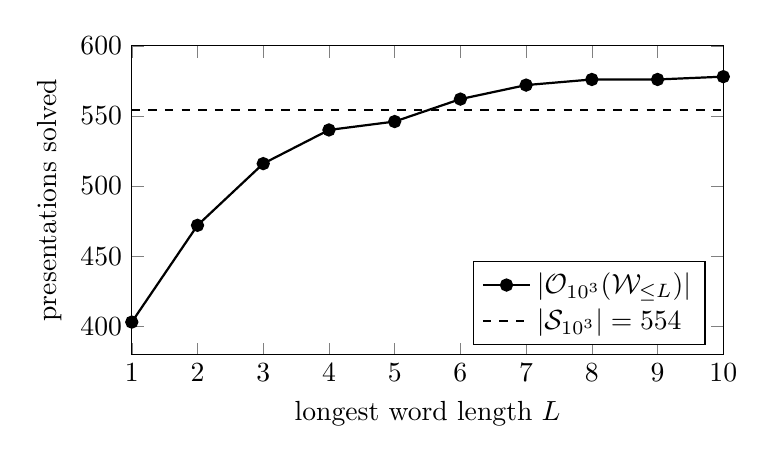
\begin{tikzpicture}
\begin{axis}[width=0.75\textwidth,height=5.5cm,xlabel={longest word length $L$},ylabel={presentations solved},
  xmin=1,xmax=10,ymin=380,ymax=600,xtick={1,...,10},legend pos=south east,legend cell align=left]
\addplot[mark=*,thick] coordinates {(1,403)(2,472)(3,516)(4,540)(5,546)(6,562)(7,572)(8,576)(9,576)(10,578)};
\addlegendentry{$|\Orc_{10^3}(\W_{\le L})|$}
\addplot[dashed,thick] coordinates {(1,554)(10,554)};
\addlegendentry{$|\Sol_{10^3}|=554$}
\end{axis}
\end{tikzpicture}
\end{center}

\noindent The measurements give the following statements for $B=10^3$.
\begin{enumerate}
  \item A uniformly random pair $(P,w)$ with $|w|\le10$ is solved with probability $65.8\%$, against $554/640=86.6\%$
  for the rank-2 search. On the $554$ presentations of $\Sol$, the rank-3 search needs fewer pops than the rank-2
  search in $0.59\%$ of the pairs, more pops in $75.4\%$, and fails within the budget in $24.0\%$.
  \item When both searches succeed, the rank-3 search pops a median of $2.00$ times as many states as the rank-2 search.
  The geometric mean of the ratio is $2.53$ and the mean excess is $110.6$ pops.
  \item Charging a failure the full budget, the expected number of pops of a random rank-3 start is $2.06$ times that of
  the rank-2 search over MS640, and $4.56$ times over the $554$ presentations of $\Sol$.
  \item The oracle exceeds the rank-2 score only for $L\ge6$. It reaches $578$ ($24$ gained, $0$ lost) at $L=10$, while
  $|\W_{\le L}|$ grows by a factor of $3$ per unit of $L$.
  \item $\max_{w}|\Fix(w)|=528$, attained by $w=\texttt{yXYYYxyyy}$; no word attains $554$. A word selected on one half
  of MS640 and scored on the other half solves $258$ and $264$ of $320$, against $281$ and $273$ for the rank-2 search.
  \item All $24$ gained presentations lie in $\Sol_{B'}$ for some $B'\le26{,}838$ ($20$ of them for $B'\le10^4$).
  Enumerating $\W_{\le10}$ in shortlex order until a word succeeds costs at least $41{,}711$ pops on each of them.
\end{enumerate}

\paragraph{Score at $B=10^4$, words of length $1$ to $7$} ($2{,}186$ words, $1{,}399{,}040$ searches;
$|\Sol|=606$).
\begin{center}
\begin{tabular}{lrr}
\toprule
& $B=10^3$ & $B=10^4$\\
\midrule
rank-2 score $|\Sol_B|$ & $554$ & $606$\\
oracle $|\Orc_B(\W_{\le7})|$ & $572$ & $608$\\
gained / lost & $20$ / $2$ & $6$ / $4$\\
best single word $\max_w|\Fix_B(w)|$ & $512$ & $572$\\
random pair solved & $66.5\%$ & $80.9\%$\\
on $\Sol_B$: fewer / more / unsolved & $0.70$ / $76.1$ / $23.2\%$ & $0.85$ / $84.5$ / $14.7\%$\\
median node ratio (both solve) & $1.80$ & $2.00$\\
expected pops relative to rank 2 (all / on $\Sol_B$) & -- & $2.74$ / $5.24$\\
\bottomrule
\end{tabular}
\end{center}
Increasing the budget by a factor of $10$ reduces the oracle's margin over the rank-2 search from $18$ presentations to
$2$. With a fixed word for every row at $B=5\cdot10^5$, the choices $w=r_1,r_2,x,y$ solve $619$, $602$, $540$ and $523$
presentations, against $638$ for the rank-2 search.

\paragraph{Validity.}
\begin{itemize}
  \item \emph{Cap.} The cap discarded a child in $2{,}331{,}711$ of the $40{,}098{,}032$ searches of the study (ranks $3$
  to $5$, both budgets). In none of them does the condition of Remark~\ref{rem:budget}(2) fail, so every score holds
  for every cap $c\ge24$.
  \item \emph{Relabelling.} MS640 consists of $319$ presentations up to the renaming of $x,y$, each listed two or four
  times. Between two copies, the node count of a rank-3 search differs by more than $14$--$21\%$ in one pair in ten, and
  the outcome differs in at most $1.8\%$ of pairs. Counting each class once, the rank-2 search solves $276/319$ and the
  oracle $288/319$ ($12$ gained, $0$ lost).
  \item \emph{Verification.} Every stored path (more than $120{,}000$) was replayed by a separate implementation, and
  $2{,}570$ stored results were recomputed with a reference solver, with $0$ mismatches. Seven independent checking
  programs, written from a prose specification, reported $0$ mismatches.
  \item \emph{Cost.} $1{,}329$ core-hours ($0.13$ core-seconds per search) at $B=10^3$, $L\le10$; $354$ core-hours at
  $B=10^4$, $L\le7$.
\end{itemize}

\subsubsection{n-generators search}

\paragraph{(a) Several stabilising words.} Take $k=2$ and $k=3$ in Definition~\ref{def:start}, with every unordered
$k$-tuple of words, repetitions allowed, at $B=10^3$. Each row is compared with rank $3$ on the same word pool.

\begin{center}
\small
\begin{tabular}{lrrrr}
\toprule
& rank 3, $\W_{\le3}$ & rank 4, $\W_{\le3}^2$ & rank 3, $\W_{\le2}$ & rank 5, $\W_{\le2}^3$\\
\midrule
starts per presentation & 26 & 351 & 8 & 120\\
random start solved & 68.7\% & 59.1\% & 66.3\% & 53.6\%\\
on $\Sol$: fewer pops & 0.75\% & 0.18\% & 0.97\% & 0.05\%\\
on $\Sol$: unsolved & 20.6\% & 31.7\% & 23.4\% & 38.1\%\\
geometric-mean node ratio & 2.31 & 3.51 & 2.16 & 3.59\\
oracle (rank 2: $554$) & 516 & 506 & 472 & 416\\
gained / lost & 0 / 38 & 0 / 48 & 0 / 82 & 0 / 138\\
best single start & 478 & 454 & 449 & 376\\
\bottomrule
\end{tabular}
\end{center}

On an equal word pool, each additional generator lowers the oracle score, the success probability of a random start
and the score of the best single start. It also raises the node ratio.

\paragraph{(b) Transformation to short relators.}
\begin{definition}[Definition step and triangulation]
Let $d=ab$ be a cyclic digram occurring in $R$. The \emph{definition} $h:=d$ adds a generator $h$ and the relator
$d^{-1}h$, and rewrites each relator by replacing occurrences of $d$ by $h$ (and $d^{-1}$ by $h^{-1}$) wherever this
shortens it. \emph{Triangulation} applies definitions while some relator has length greater than $3$, each time choosing
the digram with the most cyclic occurrences.
\end{definition}

\begin{lemma}
Triangulation terminates, and its output $\tau(P)$ satisfies
\[\tau(P)\ \text{AC-trivial}\;\Longrightarrow\;P\ \text{stably AC-trivial}.\]
\end{lemma}

\begin{proof}
Each definition shortens a relator of length greater than $3$, so the excess $\sum_i\max(0,|r_i|-3)$ strictly
decreases. Each definition is an AC4 move followed by the automorphism $h\mapsto d^{-1}h$ (as in
Proposition~\ref{prop:stab}) and AC moves.
\end{proof}

The code lifts a solution of the root $\tau(P)$ to elementary stable moves on $P$ and replays them. On MS640 the
root has rank $4$ to $11$ (mean $6.99$).

\paragraph{Score.} At $B=10^4$, cap $24$, the search on $\tau(P)$ solves $298/640$ of MS640 against $606$ for the
rank-2 search, and $8/60$ of bench60 against $40$. Every presentation solved through $\tau(P)$ is also solved at rank
$2$. The lifted certificates have a median of $690.5$ elementary moves (maximum $2{,}230$).

\paragraph{(c) Rank changes during the search.} The hybrid solver interleaves definition steps (rank $n\to n+1$) and
elimination steps with the rank-2 search. An elimination solves for a generator occurring once in a relator and
substitutes it ($n\to n-1$). Its budget is $10^3$ \emph{work units}, which are not pops, so its scores are not
comparable with the tables above. It solves $640/640$ of MS640, $60/60$ of bench60, $188/188$ of ladder200 and
$72{,}779/72{,}779$ of AC19. Of the AC19 certificates, $188$ use definition or elimination steps and are therefore
stable certificates.

\subsubsection{Change of Variables (CoV)}

\begin{definition}[Change of variables]
Let $P=\pres{x,y}{r_1,r_2}$ and let $w\in\F(x,y)$.
\begin{enumerate}
  \item Stabilise to $P_w=\pres{x,y,z}{r_1,r_2,z^{-1}w}$.
  \item Replace non-overlapping occurrences of $w^{\pm1}$ in $r_1,r_2$ by $z^{\pm1}$ and freely reduce.
  \item Choose a relator in which a generator $g\in\{x,y\}$ occurs exactly once together with $z$. Write it cyclically
  as $g^{\epsilon}s$, so that $g=s^{-\epsilon}$ in the group.
  \item Substitute $g=s^{-\epsilon}$ into the other two relators and delete the chosen relator.
  \item Rename the remaining two generators as $x,y$.
\end{enumerate}
The result is a rank-2 presentation $P'$, the \emph{image}, and $P'$ is searched with the unchanged rank-2 greedy.
\end{definition}

\begin{lemma}
If the image $P'$ is AC-trivial, then $P$ is stably AC-trivial. If, in addition, $P'=\varphi(P)$ for some
$\varphi\in\Aut(\F_2)$ up to AC moves, then $P$ is AC-trivial.
\end{lemma}

\begin{proof}
Step 1 is Proposition~\ref{prop:stab}. Steps 2--4 are AC moves on $P_w$ followed by AC5 after an automorphism that
isolates $g$. The second statement is Lemma~\ref{lem:aut}.
\end{proof}

The default family takes $w$ among the cyclic subwords of length at least $2$ of the relators. It discards any $w$
whose substitution leaves a relator of length at most $2$. The \emph{one-shot policy} searches $P$ first and then the
images in a fixed order, with $10^3$ pops per image and at most $10^4$ pops in total per presentation. The exhaustive
family keeps every proper cyclic subword and every set of non-overlapping occurrences, with one image per class under
relator order, rotation, inversion and the $8$ signed permutations: $114{,}042$ images over MS640.

\paragraph{Score of the one-shot policy} ($10^3$ pops per image, $10^4$ per presentation) against the rank-2 greedy at
$B=10^4$:
\begin{center}
\begin{tabular}{lrrr}
\toprule
set & CoV & of which stable certificates & LENGTH greedy\\
\midrule
MS640 & $584$ & $30$ & $606$\\
bench60 & $39$ & $10$ & $40$\\
ladder200 & $92$ & $48$ & $40$\\
\bottomrule
\end{tabular}
\end{center}
At equal total pops the policy scores below the rank-2 greedy on MS640 and bench60, and above it on ladder200, whose
rows are graded by the cost of the LENGTH greedy.

\paragraph{Score of the exhaustive oracle on MS640.} Each of the $114{,}042$ images is searched with the full budget.
\begin{center}
\begin{tabular}{rrrrr}
\toprule
budget & rank-2 & oracle & oracle & mean pops per presentation\\
per image & $|\Sol_B|$ & & $-$ rank 2 & to search all images\\
\midrule
$10^2$ & $455$ & $555$ & $100$ & $5{,}328.4$\\
$10^3$ & $554$ & $604$ & $50$ & --\\
$10^4$ & $606$ & $626$ & $20$ & $164{,}758.7$\\
$10^5$ & $634$ & $640$ & $6$ & $657{,}198.0$\\
\bottomrule
\end{tabular}
\end{center}
At $B=10^4$, a uniformly random image of a presentation needs fewer pops than the rank-2 search in $33.0\%$ of the
pairs, the same number in $9.6\%$, more in $48.3\%$, and fails in $9.2\%$. The $20$ presentations gained at $10^4$
coincide with the $20$ presentations that $\SMK$ solves and LENGTH does not.

\emph{Cap.} Images were searched at cap $\max(24,\ \text{longest relator}+16)$ (between $24$ and $91$), the rank-2
search at cap $24$. The comparison therefore favours CoV.

\paragraph{CoV against the rank-3 start on the same words.} With $w$ ranging over the proper cyclic subwords of the
relators, the oracle of the rank-3 start solves $544$ at $B=10^3$ and $592$ at $B=10^4$, against $604$ and $626$ for
the CoV images built from the same words. Every presentation solved by the rank-3 start is also solved by CoV. The two
constructions differ only in the elimination of a generator after the substitution, which therefore accounts for a
difference of $60$ presentations at $B=10^3$ and $34$ at $B=10^4$.

\subsection{Automorphisms}

\begin{definition}[Whitehead automorphisms and canonical form]
The Whitehead automorphisms of $\F_2$ are the $8$ signed permutations of $\{x,y\}$ together with $12$ automorphisms of
the second kind, such as $x\mapsto xy$. \emph{Peak reduction} applies Whitehead automorphisms that lower $\lambda$
until none does. The \emph{canonical form} of $P$ is the lexicographic minimum of the set of presentations of minimal
total length in its orbit. It is a complete invariant of the $\Aut(\F_2)$-orbit of $P$ modulo the state equivalence.
\end{definition}

\begin{proposition}[Transport]
Let $\varphi\in\Aut(\F_2)$ and let $\gamma$ be a sequence of AC moves from $\varphi(P)$ to $T_2$. Then $\varphi^{-1}$
applied move by move to $\gamma$, followed by the Nielsen moves of a factorisation of $\varphi$ into Whitehead
automorphisms, is a sequence of AC moves from $P$ to $T_2$.
\end{proposition}

\begin{proof}
This is the proof of Lemma~\ref{lem:aut}, applied with $\varphi^{-1}$. An S-move is mapped to the S-move whose
conjugators are the images of the original conjugators.
\end{proof}

The \emph{aut} method searches the canonical form of $P$ with $\SMK$ and transports the solution back to $P$. Its
certificates are AC certificates on $P$.

\paragraph{Score.}
\begin{itemize}
  \item \emph{Orbit counts.} MS640 contains $113$ orbits, the $156{,}762$ extended AC19 presentations contain
  $72{,}779$, and the $1{,}136{,}154$ AC1M presentations contain $71{,}283$.
  \item \emph{The aut method} at $B=10^4$, cap $24$, solves $626/640$ of MS640 ($11$ plain and $615$ transported
  certificates) and $52/60$ of bench60. These equal the $\SMK$ scores on the input presentations.
  \item \emph{The canonical form need not be easier.} On the original presentations of the $40$ hardest AC19 orbits,
  the LENGTH greedy solves $40/40$ (median $5{,}720$ pops, maximum $52{,}143$) and $\SMK$ solves $18/18$. Within
  $10^7$ pops, none of their canonical representatives is solved ($0/28$ with LENGTH, $0/9$ with $\SMK$).
  Minimisation shortens the input on $34$ of the $40$ presentations and raises the peak length on all $40$ (median
  $29$ to $49$).
  \item \emph{Transport.} All $58$ transported certificates replay on the representatives, with every one of the
  $2{,}211$ and $1{,}069$ transported steps equivariant.
\end{itemize}

\end{document}
